\documentclass[svgnames,hyperref={bookmarks=false}]{beamer}
\useoutertheme{infolines}
\setbeamertemplate{headline}{} % removes the headline that infolines inserts
% \setbeamertemplate{footline}{
%   \hfill%
%   \usebeamercolor[fg]{page number in head/foot}%
%   \usebeamerfont{page number in head/foot}%
%   \insertpagenumber\,/\,\insertpresentationendpage\kern1em\vskip2pt%
% }
\setbeamertemplate{footline}{
  \hfill%
  \usebeamercolor[fg]{page number in head/foot}%
  \usebeamerfont{page number in head/foot}%
  \footnotesize\insertpagenumber\kern1em\vskip2pt%
}
\setbeamertemplate{navigation symbols}{}
\setbeamercolor{alerted text}{fg=blue}
\setbeamerfont{alerted text}{series=\bfseries,family=\ttfamily}
\setbeamertemplate{section in toc}{\text{\color{black}{\inserttocsection}}}
\usepackage[parfill]{parskip}
\usepackage[linewidth=0.5pt]{mdframed}
\newmdenv[innerleftmargin=1mm, innerrightmargin=1mm, innertopmargin=-1mm, innerbottommargin=2mm, leftmargin=-1mm, rightmargin=-1mm]{lstlistinglike}
\usepackage{tikz}
\usepackage{graphicx}
\usepackage{pdfpages}
\DeclareGraphicsExtensions{.pdf,.png,.jpg}
\usepackage{textcomp}
\usepackage{pifont}
\usepackage{tabu}
\usepackage{fancyvrb}

% The following \documentclass options may be useful:
%
% 10pt          To set in 10-point type instead of 9-point.
% 11pt          To set in 11-point type instead of 9-point.
% authoryear    To obtain author/year citation style instead of numeric.

\usepackage{amsmath}
\usepackage{amssymb}

%\usepackage{fleqn}
\usepackage{listings}
\usepackage{math}
\usepackage{amsmath}
\usepackage{latexsym}
\usepackage{bcprules}
%\usepackage[scaled=0.848971]{luximono} % This is for 11 pt Default font
\usepackage[T1]{fontenc}

% Prooftree formatting
\usepackage{prooftree}

\usepackage{multicol}
\usepackage{framed}

\usepackage{stmaryrd}

%\usepackage{float}
%\floatstyle{boxed}
%\restylefloat{figure}

% support for generating PDF files
%\newif\ifpdf
%    \ifx\pdfoutput\undefined
%    \pdffalse
%\else
%    \pdftrue
%    \pdfoutput=1
%\fi

%versions
% Use dependent function types
\newif\ifdep\depfalse

\lstset{
  literate=
  {=>}{$\Rightarrow\;$}{2}
  {<:}{$<:\;$}{1}
}

\lstdefinelanguage{scala}{%
       morekeywords={%
                try, catch, throw, private, public, protected, import, package, implicit, final, package, trait, type, class, val, def, var, if, for, this, else, extends, with, while, new, abstract, object, case, match, sealed,override},
         sensitive=t, %
   morecomment=[s]{/*}{*/},morecomment=[l]{\//},%
   mathescape,
%   escapeinside={/*\%}{*/},%
   rangeprefix= /*< ,rangesuffix= >*/,%
   morestring=[d]{"}%
 }

\lstset{breaklines=true,language=scala}

\def\code{\lstinline}  % shorter version so you can write \code|String[Foo]|
                       % -- \def must be in same file as uses for this to
                       % work...
\newcommand{\lstref}[1]{Listing~\ref{#1}}
\newcommand{\Lstref}[1]{Listing~\ref{#1}} % only capitalise at beginning of sentence?
\newcommand{\secref}[1]{Section~\ref{#1}}
\newcommand{\Secref}[1]{Section~\ref{#1}} % only capitalise at beginning of sentence?



% \lstset{basicstyle=\footnotesize\ttfamily, breaklines=true, language=scala, tabsize=2, columns=fixed, mathescape=false,includerangemarker=false}
% thank you, Burak
% (lstset tweaking stolen from
% http://lampsvn.epfl.ch/svn-repos/scala/scala/branches/typestate/docs/tstate-report/datasway.tex)
\lstset{
    xleftmargin=2em,%
    framesep=5pt,%
    frame=none,%
    captionpos=b,%
    fontadjust=true,%
    columns=[c]fixed,%
    keepspaces=false,%
    basewidth={0.56em, 0.52em},%
    tabsize=2,%
    basicstyle=\small\tt,% \small\tt
    commentstyle=\textit,%
    keywordstyle=\bfseries,%
    escapechar=\%,%
}

%% set latex/pdflatex specific stuff
%\ifpdf
%    \usepackage[pdftex,
%                hyperindex,
%                plainpages=false,
%                breaklinks,
%                colorlinks,
%                citecolor=black,
%                filecolor=black,
%                linkcolor=black,
%                pagecolor=black,
%                urlcolor=black]{hyperref}
%    \usepackage[pdftex]{graphicx}
%    \DeclareGraphicsExtensions{.png,.pdf}
%    \pdfcatalog {
%        /PageMode (/UseNone)
%    }
%    \usepackage{thumbpdf}
%    \usepackage[pdftex]{color}
%\else
%    \usepackage[ps2pdf]{hyperref}
%    \usepackage{graphicx}
%    \DeclareGraphicsExtensions{.eps,.jpg}
%    \usepackage{color}
%\fi

%\setlength{\parindent}{0pt}
%\setlength{\parskip}{5pt}

% verbfilter stuff
\newcommand{\prog}[1]{{\sl #1}}
\newenvironment{program}[1][10.5]
  {\fontsize{#1}{13.6}\tt\begin{tabbing}\hspace*{0.5\parindent}\=\+\kill}
  {\end{tabbing}\noindent}
\newcommand{\blockcomment}[1]{{\color{grayPoint3}#1}}
\newcommand{\linecomment}{\color{grayPoint3}}
\newcommand{\grey}{\color{grey}}

%\newenvironment{program}{\ \ \ \ \begin{minipage}{\textwidth}\renewcommand{\baselinestretch}{1.0}\sl\begin{tabbing}}{\end{tabbing}\end{minipage}}
\newcommand{\vem}{\bfseries}
\newcommand{\quotedstring}[1]{{#1}}
\newcommand{\typename}[1]{{#1}}
\newcommand{\literal}[1]{{#1}}

% comments and notes
\newcommand{\comment}[1]{}
%\newcommand{\note}[1]{{\bf $\clubsuit$ #1 $\spadesuit$}}

% figures
\newcommand{\figurebox}[1]
        {\fbox{\begin{minipage}{\textwidth} #1 \medskip\end{minipage}}}
%        {\fbox{\begin{minipage}{\textwidth}\begin{center} #1 \end{center}\medskip\end{minipage}}}
\newcommand{\boxfig}[3]
        {\begin{figure*}\figurebox{#3\caption{\label{fig:#1}#2}}\end{figure*}}
\newcommand{\figref}[1]
        {Figure~\ref{fig:#1}}

% typing rules (not used here)
\newcommand{\ttag}[1]{\mbox{\textsc{\small(#1)}}}
\newcommand{\infer}[3]{\mbox{#1 }\ba{c} #2 \\ \hline #3 \ea}
\newcommand{\irule}[2]{{\renewcommand{\arraystretch}{1.2}\ba{c} #1
                        \\ \hline #2 \ea}}
\newlength{\trulemargin}
\newlength{\trulewidth}
\newlength{\srulewidth}
\setlength{\trulemargin}{0.80cm}
\setlength{\trulewidth}{40.0mm}
\setlength{\srulewidth}{3.0cm}
\newenvironment{trules}{$\vspace{0.5em}\ba{p{\trulemargin}@{~}p{\trulewidth}@{~}p{\trulemargin}}}{\ea$}
\newenvironment{srules}{$\vspace{0.5em}\ba{p{\trulemargin}@{~}p{\srulewidth}}}{\ea$}
\newcommand{\laxiom}[2]{\ttag{#1} & $ #2 \hfill\ }
\newcommand{\raxiom}[2]{\hfill #2 $& \hfill \ttag{#1}}
\newcommand{\caxiom}[2]{\ttag{#1} & $\hfill #2 \hfill $& \ }
\newcommand{\lrule}[3]{\laxiom{#1}{\irule{#2}{#3}}}
\newcommand{\rrule}[3]{\raxiom{#1}{\irule{#2}{#3}}}
\newcommand{\crule}[3]{\caxiom{#1}{\irule{#2}{#3}}}
\newcommand{\lsrule}[3]{\lsaxiom{#1}{\irule{#2}{#3}}}
\newcommand{\rsrule}[3]{\rsaxiom{#1}{\irule{#2}{#3}}}
\newcommand{\nl}{\end{trules}\\[0.5em] \begin{trules}}
\newcommand{\snl}{\end{srules}\\[0.5em] \begin{srules}}

% commas and semicolons
\newcommand{\comma}{,\,}
\newcommand{\commadots}{\comma \ldots \comma}
\newcommand{\semi}{;\mbox{;};}
\newcommand{\semidots}{\semi \ldots \semi}

% math stuff
\newenvironment{myproof}{{\em Proof:}}{$\Box$}
\newenvironment{proofsketch}{{\em Proof Sketch:}}{$\Box$}
\newcommand{\Case}{{\em Case\ }}

% make ; a delimiter in math mode
% \mathcode`\;="8000 % Makes ; active in math mode
% {\catcode`\;=\active \gdef;{\;}}
% \mathchardef\semicolon="003B

% reserved words
\newcommand{\mathem}{\bf}

% brackets
\newcommand{\set}[1]{\{#1\}}
\newcommand{\sbs}[1]{\lquote #1 \rquote}

% arrays
\newcommand{\ba}{\begin{array}}
\newcommand{\ea}{\end{array}}
\newcommand{\bda}{\[\ba}
\newcommand{\eda}{\ea\]}
\newcommand{\ei}{\end{array}}
\newcommand{\bcases}{\left\{\begin{array}{ll}}
\newcommand{\ecases}{\end{array}\right.}

% \cal ids
\renewcommand{\AA}{{\cal A}}
\newcommand{\BB}{{\cal B}}
\newcommand{\CC}{{\cal C}}
\newcommand{\DD}{{\cal D}}
\newcommand{\EE}{{\cal E}}
\newcommand{\FF}{{\cal F}}
\newcommand{\GG}{{\cal G}}
\newcommand{\HH}{{\cal H}}
\newcommand{\II}{{\cal I}}
\newcommand{\JJ}{{\cal J}}
\newcommand{\KK}{{\cal K}}
\newcommand{\LL}{{\cal L}}
\newcommand{\MM}{{\cal M}}
\newcommand{\NN}{{\cal N}}
\newcommand{\OO}{{\cal O}}
\newcommand{\PP}{{\cal P}}
\newcommand{\QQ}{{\cal Q}}
\newcommand{\RR}{{\cal R}}
\newcommand{\TT}{{\cal T}}
\newcommand{\UU}{{\cal U}}
\newcommand{\VV}{{\cal V}}
\newcommand{\WW}{{\cal W}}
\newcommand{\XX}{{\cal X}}
\newcommand{\YY}{{\cal Y}}
\newcommand{\ZZ}{{\cal Z}}

%\newcommand{\inst}{\mbox{\mathem inst}}
\newcommand{\trans}[1]{\la\!\la#1\ra\!\ra}
\newcommand{\remark}[1]{{\bf $\clubsuit$ #1 $\spadesuit$}}
\newcommand{\todo}[1]{\remark{to do: #1}}
%\newcommand{\J}{\justifies}
%\newcommand{\U}{\using}

% names
\newcommand{\Scala}{\mbox{\textsc{Scala}}}
\newcommand{\Java}{\mbox{\textsc{Java}}}

%\renewcommand\textfraction{.05}
%\renewcommand\floatpagefraction{.9}
%\renewcommand\topfraction{.8}


%%%%%%%%%%%%%%%%%%%%%%%%%%%%%%%%%%%%%%%
%   Language abstraction commands     %
%%%%%%%%%%%%%%%%%%%%%%%%%%%%%%%%%%%%%%%

% spacing
\newcommand{\gap}{\quad\quad}
\newcommand{\biggap}{\quad\quad\quad}
\newcommand{\nextline}{\\ \\}
\newcommand{\htabwidth}{0.5cm}
\newcommand{\tabwidth}{1cm}
\newcommand{\htab}{\hspace{\htabwidth}}
\newcommand{\tab}{\hspace{\tabwidth}}
\newcommand{\linesep}{\ \hrulefill \ \smallskip}

\newcommand{\mi}[1]{\mathit{#1}}

% misc symbols
\newcommand{\dhd}{\!\!\!\!\!\rightarrow}
\newcommand{\Dhd}{\!\!\!\!\!\Rightarrow}
\newcommand{\ts}{\,\vdash\,}
\newcommand{\la}{\langle}
\newcommand{\ra}{\rangle}
\newcommand{\eg}{{\em e.g.}}

% misc identifiers
\newcommand{\dom}{\mbox{\sl dom}}
\newcommand{\fn}{\mbox{\sl fn}}
\newcommand{\bn}{\mbox{\sl bn}}
\newcommand{\sig}{\mbox{\sl sig}}
\newcommand{\IF}{\mbox{\mathem if}}
\newcommand{\OTHERWISE}{\mbox{\mathem otherwise}}
\newcommand{\expand}{\prec}
\newcommand{\weakexpand}{\prec^W}
\newcommand{\spcomma}{~,~}

%% Relations
% Subtype 
\newcommand{\sub}{<:}
% Type assignment
\newcommand{\typ}{:}
% reduction
\newcommand{\reduces}{\;\rightarrow\;}
% well-formedness
\newcommand{\wf}{\;\mbox{\textbf{wf}}}
\newcommand{\nswf}{\mbox{\textbf{wf}}}
\newcommand{\wfe}{\;\mbox{\textbf{wfe}}}
\newcommand{\nswfe}{\mbox{\textbf{wfe}}}

%% Operators
% Type selection
\newcommand{\tsel}{\#}
% Function type
\newcommand{\tfun}{\rightarrow}
\newcommand{\dfun}[3]{(#1\!:\!#2) \Rightarrow #3}
% Conjunction
\newcommand{\tand}{\wedge}
% Disjunction
\newcommand{\tor}{\vee}
% Singleton type suffix
\newcommand{\sing}{.\textbf{type}}

%% Syntax
% Header for typing rules
\newcommand{\judgement}[2]{{\bf #1} \hfill #2}
% Widening
\newcommand{\wid}[2]{#1 : #2}
% Refinement
\newcommand{\refine}[2]{\left\{#1 \Rightarrow #2 \right\}}
\newcommand{\mlrefine}[2]{\{#1 \Rightarrow #2 \}}
% Field definitions
\newcommand{\ldefs}[1]{\left\{#1\right\}}
\newcommand{\mlldefs}[1]{\{#1\}}
% Member sequences
\newcommand{\seq}[1]{\overline{#1}}
% Lambda
\newcommand{\dabs}[3]{(#1\!:\!#2)\Rightarrow #3}
\newcommand{\abs}[3]{\lambda #1\!:\!#2.#3}
% Method Application
\newcommand{\mapp}[3]{#1.#2(#3)}
% Substitution
\newcommand{\subst}[3]{[#1/#2]#3}
% Object creation
\newcommand{\new}[3]{\textbf{val }#1 = \textbf{new }#2 ;\; #3}
\newcommand{\mlnew}[3]{\textbf{val }#1 = \textbf{new }#2 ;\;\\&#3}
%\renewcommand{\new}[3]{#1 \leftarrow #2 \,\textbf{in}\, #3}
% Field declaration
\newcommand{\Ldecl}[3]{#1 : #2..#3}%{#1 \operatorname{>:} #2 \operatorname{<:} #3}
\newcommand{\ldecl}[2]{#1 : #2}
\newcommand{\mdecl}[3]{#1 : #2 \tfun #3}
% Top and Bottom
\newcommand{\Top}{\top}%{\textbf{Top}}
\newcommand{\Bot}{\bot}%\textbf{Bot}}
% Environment extension
%\newcommand{\envplus}[1]{\uplus \{ #1 \}}
\newcommand{\envplus}[1]{, #1}
% Reduction
\newcommand{\reduction}[4]{#1 \operatorname{|} #2 \reduces #3 \operatorname{|} #4}

% Sugar
\newcommand{\arrow}[2]{#1\rightarrow_s#2}
\newcommand{\fun}[4]{\textbf{fun } (#1:#2)\;#3\;#4}
\newcommand{\app}[2]{(\textbf{app }#1\;#2)}
\newcommand{\mlapp}[2]{(\textbf{app }#1\;\\&#2)}
\newcommand{\cast}[2]{(\textbf{cast }#1\;#2)}

\newcommand{\lindent}{\hspace{-4mm}}

% Logical relations
\newcommand{\relv}[4]{\mathcal{V}_{#1;#2;#3}\llbracket#4\rrbracket}
\newcommand{\rele}[4]{\mathcal{E}_{#1;#2;#3}\llbracket#4\rrbracket}
\newcommand{\rels}[3]{\mathcal{\supseteq}_{#1}\llbracket#2;#3\rrbracket}
\newcommand{\relg}[3]{\mathcal{\supseteq^!}_{#1;#2}\llbracket#3\rrbracket}
\newcommand{\irred}[2]{\text{irred }(#1,#2)}
\newcommand{\andl}{\;\wedge\;}
\newcommand{\orl}{\vee}
\newcommand{\impliesl}{\rightarrow}
\newcommand{\reductionl}[5]{#1 \operatorname{|} #2 \;\rightarrow^{#5}\; #3 \operatorname{|} #4}
\newcommand{\ds}{\,\vDash\,}


\begin{document}
\newcommand{\rts}{\ \dashv\ }

% eugene:
%
% like
% not your typical
% tofte talpin how to pronounce
% {r} explain
% merge 7, 8 or make {r} a comment
% regions: coloring for new stuff
% better explanatino of qualifiers (examples?)
% better arrows for isolated+immutable picture
% too much update/collection-cycle explanations
% snapshot
%   heap state -> heap address
%   time       -> observed time
% too much text research proposal part
% opaque pronounciation
% extra slides to replace questions
%
% dima:
%
% explain region open vs evidence
% explain when region evidence is not needed
% consider reordering reference qualifiers: swap immutable and writable
% explain isolated-immutable reference
% 4 nulls
% explain RemIso
% remiso
% no synchronization in write barrier, not no synchronization at all
% new slide! explain when to deallocate separate slide
% explain _i == thread number i
% ownership vs regions about the same?
% comparison table message not clear
% too much discussion summary

\title{Safe Low-Overhead Memory Management for Concurrency and Parallelism}
\author{Denys Shabalin}
\date{21 July 2015}
{
\setbeamertemplate{footline}{}
\begin{frame}
    \titlepage
\end{frame}
}


\begin{frame}
    \frametitle{Overview}
    \begin{enumerate}
        \item Region-based memory in Cyclone
        \item Uniqueness and reference immutability for safe parallelism
        \item An efficient on-the-fly cycle collection
        \item Research proposal
    \end{enumerate}
\end{frame}

\begin{frame}
    \begin{center}
        {\LARGE Region-based memory in Cyclone} \\
        \vspace{20pt}
        Dan Grossman, Michael Hicks, Greg Morrisett,\\
        Yanling Wang, Trevor Jim, James Cheney
    \end{center}
\end{frame}

\begin{frame}
    \frametitle{Safe region-based memory management}

    Pioneered by M. Tofte and J.P. Talpin who explored the concept in functional
    programming languages of the ML family.
\end{frame}

\begin{frame}
    \frametitle{Cyclone overview}
    \begin{itemize}
        \item Close to C syntactically to ease porting of existing programs.
        \item Adds tagged unions, polymorphism, \textit{regions} etc.
        \item Guarantees memory safety via static type checking.
    \end{itemize}
\end{frame}

\begin{frame}[fragile]
    \frametitle{Regions in Cyclone}
    \begin{verbatim}
    void main() {
        region r {
            struct Point*r p = rnew(r) { 10.0, 10.0 };
            printf("Point at (%d, %d)", p->x, p->y);
        }
    }
    \end{verbatim}
\end{frame}

\begin{frame}[fragile]
    \frametitle{Regions in Cyclone}
    \begin{verbatim}
    void main() {
        region r {
            struct Point*r p = rnew(r) { 10.0, 10.0 };
            printPoint<r>(p)
        }
    }

    void printPoint<r>(Point*r p) {
        printf("Point at (%d, %d)", p->x, p->y);
    }
    \end{verbatim}
\end{frame}

\begin{frame}[fragile]
    \frametitle{Regions in Cyclone}
    \begin{verbatim}
    void main() {
        region r {
            struct Point*r p = rnew(r) { 10.0, 10.0 };
            printPoint<r>(p)
        }
    }

    void printPoint<r>(Point*r p; {r}) {
        printf("Point at (%d, %d)", p->x, p->y);
    }
    \end{verbatim}
\end{frame}

\begin{frame}[fragile]
    \frametitle{Cyclone type system: abstract syntax}

    $\tau ::= \tau_1 \xrightarrow{\epsilon} \tau_2\ |
            \ \tau * \rho\ |\ handle(\rho)\ |\ ... $
    \\ \vspace{10pt}

    $e ::= x_\rho\ |\ *e\ |\ e_1(e_2)\ |\ rnew(e_1)\ e_2\ |\ ...$
    \\ \vspace{10pt}

    $s ::=  e\ |\ return\ e\ |\ s_1; s_2 |
            \ region \langle \rho \rangle\ x_\rho\ s\ |\ ...$
    \\ \vspace{10pt}

    $\Gamma ::= \bullet\ |\ \Gamma, x_\rho: \tau$
    \\ \vspace{10pt}

    $\Delta ::= \bullet\ |\ \Delta, \alpha: \kappa$
    \\ \vspace{10pt}

    $\gamma ::= \emptyset\ |\ \gamma, \epsilon <: \rho$
    \\ \vspace{10pt}

    $\epsilon ::= \alpha_1\ \cup\ \alpha_2\ \cup \ ...\ \cup\ \alpha_n \ \cup \
                  \{ \rho_1,\ ..., \rho_m \}$
    \\ \vspace{10pt}

    $C ::= \Gamma; \Delta; \gamma; \epsilon$
\end{frame}

\begin{frame}
    \frametitle{Cyclone type system: judgments}
    \begin{center}
    \begin{tabular}{c | c}
    Expression typing & $\Delta; \Gamma; \gamma; \epsilon \ts e: \tau$         \\
                      \hline
    Statement typing  & $\Delta; \Gamma; \gamma; \epsilon; \tau \ts_{stmt}\ s$ \\
                      \hline
    Region liveness   & $\gamma \ts \epsilon \Rightarrow \rho$                 \\
                      & $\gamma \ts \epsilon_1 \Rightarrow \epsilon_2$
    \end{tabular}
    \end{center}
\end{frame}

\begin{frame}
    \frametitle{Cyclone type system: typing pointer dereference}
    \infrule
    {
        \Delta; \Gamma; \gamma; \epsilon \ts e: \tau * \rho \ \ \ \
        \gamma \ts \epsilon \Rightarrow \rho
    }
    {
        \Delta; \Gamma; \gamma; \epsilon \ts *e: \tau
    }
\end{frame}

\begin{frame}
    \frametitle{Cyclone type system: typing function application}
    \infrule
    {
        \Delta; \Gamma; \gamma; \epsilon \ts
        e_1: \tau_2 \xrightarrow{\epsilon_1} \tau \ \
        \Delta; \Gamma; \gamma; \epsilon \ts
        e_2: \tau_2 \ \
        \gamma \ts \epsilon \Rightarrow \epsilon_1
    }
    {
        \Delta; \Gamma; \gamma; \epsilon \ts
        e_1 (e_2): \tau
    }
\end{frame}

\begin{frame}
    \frametitle{Cyclone: summary}

    \begin{itemize}
        \item
            Region based memory management ties memory management
            to explicitly delimited blocks of code
        \item
            Static safety is ensured through region-annotated reference
            types and simple effect checking
    \end{itemize}
\end{frame}

\begin{frame}
    \begin{center}
        {\LARGE Uniqueness and reference immutability\\ for safe parallelism} \\
        \vspace{20pt}
        Colin S. Gordon, Matthew J. Parkinson, \\
        Jared Parsons, Aleks Bromfield, Joe Duffy
    \end{center}
\end{frame}

\begin{frame}
    \frametitle{Uniqueness and reference immutability}
    Introduces reference qualifiers to the C\# language:
    \begin{itemize}
        \item \textbf{writable} T
        \item \textbf{readable} T
        \item \textbf{immutable} T
        \item \textbf{isolated} T
    \end{itemize}
\end{frame}

\begin{frame}
    \frametitle{Uniqueness and reference immutability}
    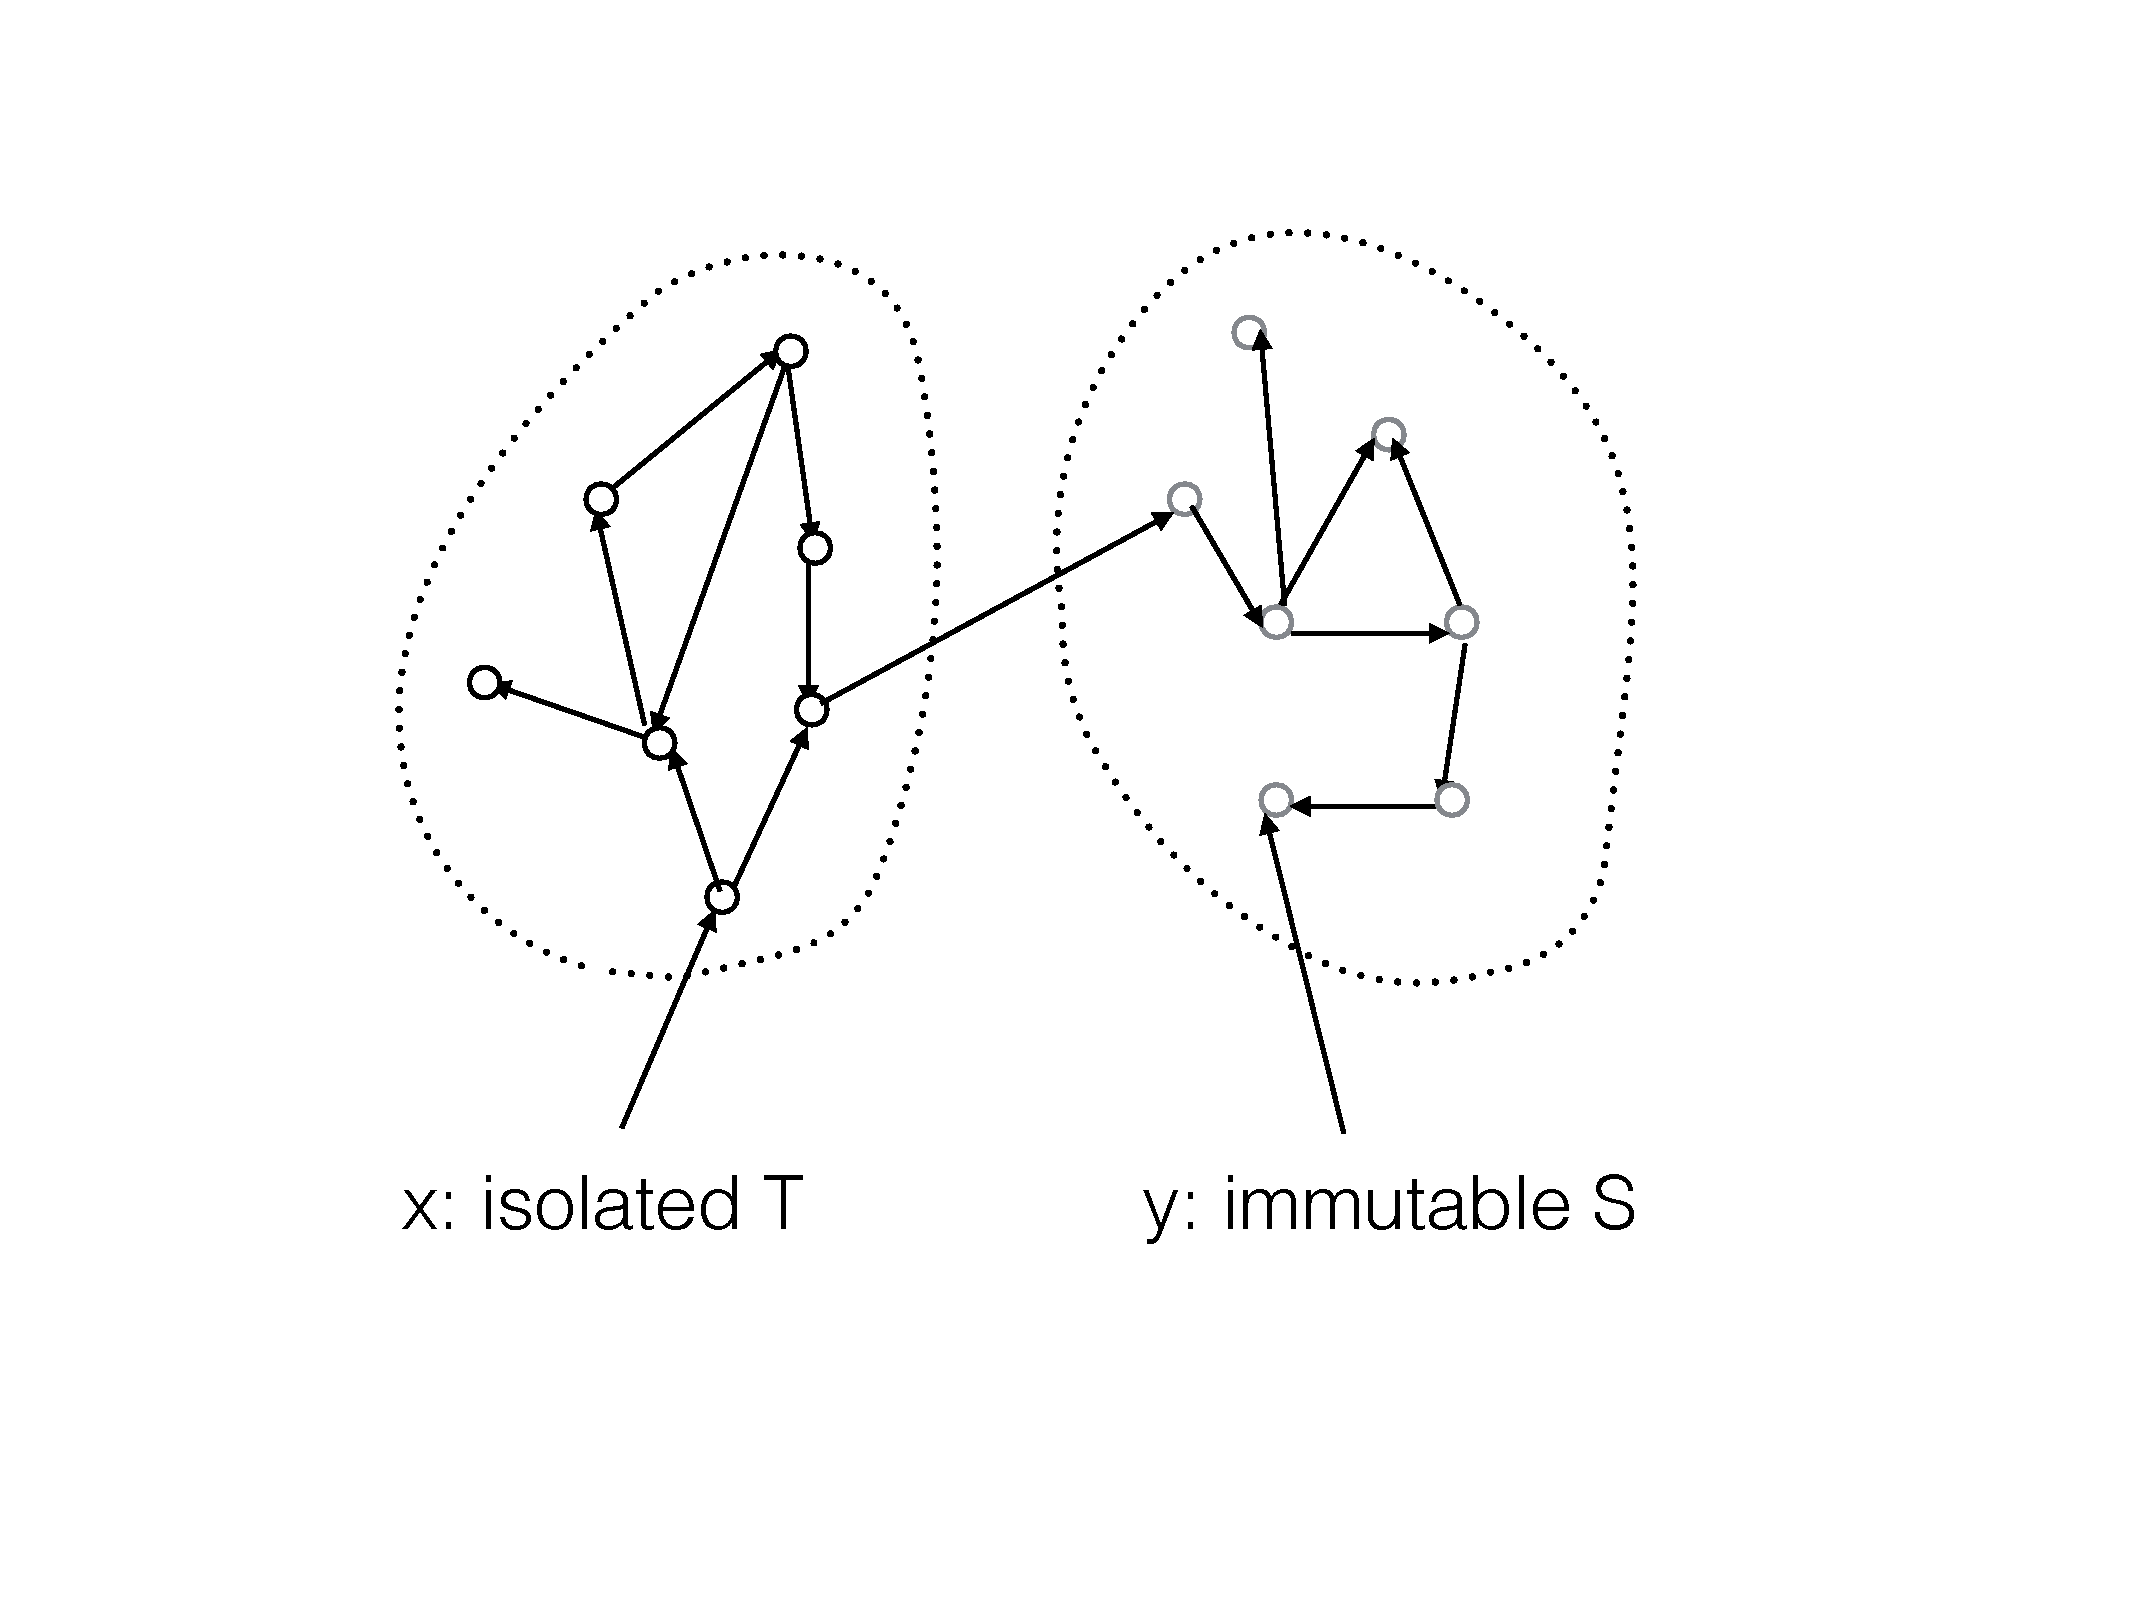
\includegraphics[width=350pt]{iso_imm.pdf}
\end{frame}

\begin{frame}
    \frametitle{Uniqueness and reference immutability: abstract syntax}

    $a ::= x = y\ |\ x.f = y\ |\ x = y.f\ |\ x = consume(y.f)\ |\ ...$

    $C ::= a\ |\ C; C\ |\ ...$

    $T ::= cn$

    $TD ::= class\ cn [<: T] \{\ fld*\ meth*\ \}$

    $p ::= readable\ |\ writable\ |\ immutable\ |\ isolated$

    $t ::= int\ |\ bool\ |\ p\ T$

    $\Gamma ::= \epsilon\ |\ \Gamma, x: t$
\end{frame}

\begin{frame}
    \frametitle{Uniqueness and reference immutability: judgements}
    \begin{center}
    \begin{tabular}{c | c}
    Command typing & $\Gamma \ts C \rts \Gamma$ \\
                   \hline

    Program typing & $\ts P$          \\
                   & $P \ts TD$       \\
                   & $P; TD \ts fld$  \\
                   & $P; TD \ts meth$ \\
                   \hline

    Subtyping & $\ts p \prec p'$    \\
              & $\ts T \prec T'$    \\
              & $\ts t_1 \prec t_2$ \\
              \hline

    Permission combination & $p_1 \rhd p_2 = p_3$                \\
                           & $p_1 \rhd p_2 T = (p_1 \rhd p_2) T$ \\
    \end{tabular}
    \end{center}
\end{frame}

\begin{frame}
    \frametitle{Uniqueness and reference immutability: typing}
    \infrule
    {
        t \neq isolated\ \_
    }
    {
        x: \_,\ y: t \ts x = y \rts y: t,\ x: t
    }
    \infrule
    {
        t'\ f \in T \\
        p \neq isolated \vee t' = immutable\ \_ \\
        t' \neq isolated\ \_ \vee p = immutable
    }
    {
        x: \_,\ y: p\ T
        \ts x = y.f
        \rts y: p\ T,\ x: p \triangleright t'
    }
    \infrule
    {
        t\ f \in T
    }
    {
        y: writable\ T,\ x: t
        \ts y.f = x
        \rts y: writable\ T,\ RemIso(x: t)
    }
    \infrule
    {
        isolated\ T_f \ f \in T
    }
    {
        y: writable\ T
        \ts x = consume(y.f)
        \rts y: writable\ T,\ x: isolated\ T
    }
\end{frame}

\begin{frame}
    \frametitle{Uniqueness and reference immutability: typing}
    \infrule
    {
        t'\ m(\seq{u'\ z'})\ p' \in T \ \ \ \
        \ts p \prec p' \ \ \ \
        \seq{\ts u \prec u'} \\
        p = isolated \Rightarrow \\
                 t \neq readable\ \_\
        \wedge\  t \neq writable\ \_\\
        \wedge\  IsoOrImm(\seq{z: t})\
        \wedge\  p' \neq immutable
    }
    {
        y: p\ T,\ \seq{z: u}
        \ts x = y.m(\seq{z})
        \rts y: p\ T,\ RemIso(\seq{z: t}),\ x: t'
    }
\end{frame}

\begin{frame}
    \frametitle{Uniqueness and reference immutability: applications}

    \begin{itemize}
        \item Statically enforced data-race freedom
        \item Optimizations of the GC due to known invariants
        \item Ownership-based memory management
    \end{itemize}
\end{frame}

\begin{frame}
    \begin{center}
        {\LARGE An efficient on-the-fly cycle collection} \\
        \vspace{20pt}
        Harel Paz, David F. Bacon, Elliot K. Kolodner,\\
        Erez Petrank, V. T. Rajan
    \end{center}
\end{frame}

\begin{frame}
    \frametitle{Efficient on-the-fly collection: previous work}
    \begin{enumerate}
        \item
            Yossi Levanoni and Erez Petrank.
            \textit{An on-the-fly reference counting garbage collection for Java}.
        \item
            David F. Bacon and V. T. Rajan.
            \textit{Concurrent cycle collection in reference counted systems}.
        \item
            Harel Paz, Erez Petrank, and Stephen M. Blackburn.
            \textit{Age-oriented concurrent garbage collection}.
    \end{enumerate}
\end{frame}

\begin{frame}
    \frametitle{1. On-the-fly ref. counting garbage collection for Java}

    Introduces two algorithms:
    \begin{enumerate}
        \item Stop-the-world snapshot algorithm
        \item On-the-fly sliding views algorithm
    \end{enumerate}
\end{frame}

\begin{frame}
    \frametitle{Stop-the-world snapshot collector}
    \begin{itemize}
        \item
            Reference counts are only heap-to-heap.
        \item
            No need to maintain reference counts between cycle collections.
            Out of multiple assignments \texttt{obj.slot = $v_1$, ..., $v_n$}
            \\ only \texttt{RC($v_1$) -= 1} and \texttt{RC($v_n$) += 1}
            are relevant.
        \item
            Instead of constantly maintaining reference counts lets
            just record old value for all of the fields that changed.
        \item
            To reclaim an object it must both have 0 reference count and
            not be referenced from stack or registers.
    \end{itemize}
\end{frame}

\begin{frame}[fragile]
    \frametitle{Stop-the-world snapshot algorithm}
    Synchronization-free write barrier:
    \begin{verbatim}

        Procedure Update(s: Slot, new: Object)
        begin
            local old := read(s)
            if not Dirty(s) then
                Buffer_i[CurrPos_i] := <s, old>
                CurrPos_i := CurrPos_i + 1
                Dirty(s) := true
            write(s, new)
        end
    \end{verbatim}
\end{frame}

\begin{frame}[fragile]
    \frametitle{Stop-the-world snapshot algorithm}
    Collector logic:
    \begin{verbatim}

        Procedure Collection-Cycle
        begin
            // Stop-The-World
            Read-Current-State
            Update-Reference-Counters
            Read-Buffers
            Fix-Undetermined-Slots
            Reclaim-Garbage
        end
    \end{verbatim}
\end{frame}

\begin{frame}
    \frametitle{On-the-fly sliding views collector}
    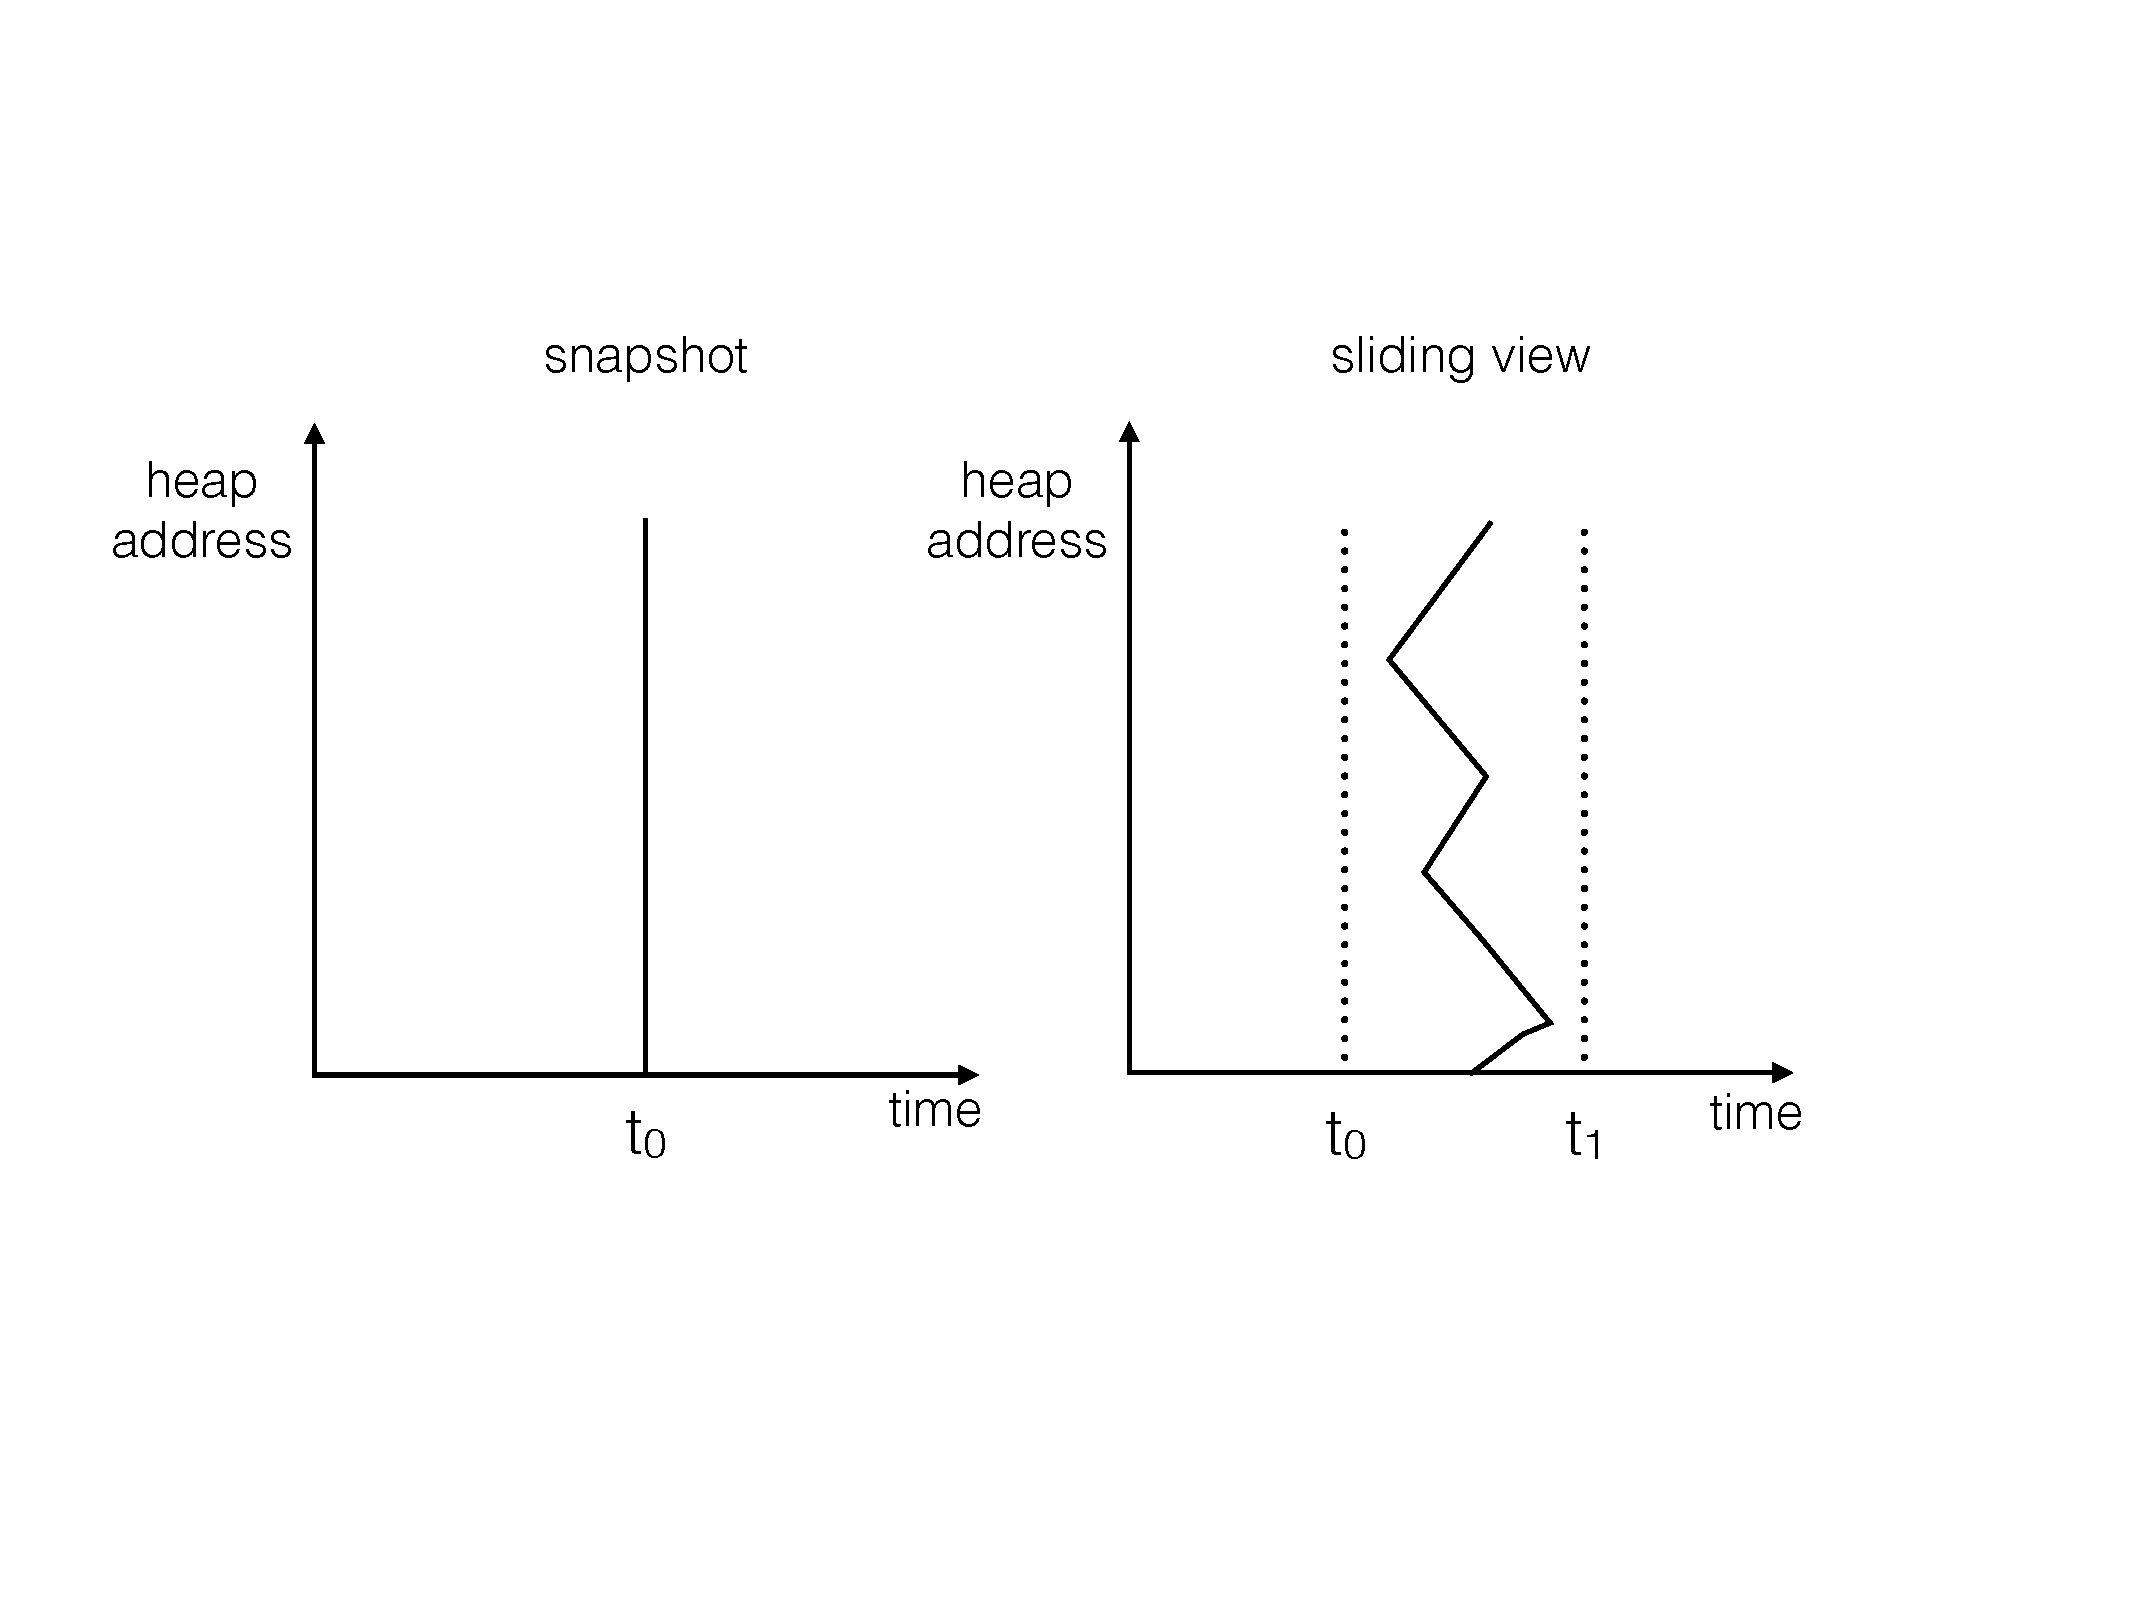
\includegraphics[width=350pt]{snapshot_sliding.pdf}
\end{frame}

\begin{frame}
    \frametitle{On-the-fly sliding views collector}
    Extra precautions needed:
    \begin{itemize}
        \item Can't collect objects to which new reference
              has been created during cycle collection.
        \item To fix this problem a \textit{snooping} mechanism is
              introduced. It effectively pins all such objects.
    \end{itemize}
\end{frame}

\begin{frame}[fragile]
    \frametitle{On-the-fly sliding views collector}
    Modified write barrier with snooping:
    \begin{verbatim}

        Procedure Update(s: Slot, new: Object)
        begin
            local old := read(s)
            if not Dirty(s) then
                Buffer_i[CurrPos_i] := <s, old>
                CurrPos_i := CurrPos_i + 1
                Dirty(s) := true
            write(s, new)
            if Snoop_i then
                Locals_i := Locals_i + new
        end
    \end{verbatim}
\end{frame}

\begin{frame}
    \frametitle{2. Concurrent cycle collection in ref. counted systems}
    \begin{itemize}
        \item
            Introduces two collectors: extremely efficient synchronization-free
            stop-the-world one and less efficient concurrent one.
        \item
            Synchronous collector cleans up the cycles starting from suspected
            cycle roots in $O(N + E)$.
        \item
            Linear performance obtained through single graph traversal
            that colors graph as it goes through it.
        \item
            Sufficient constant benefits by special treatment of acyclic
            data structures.
    \end{itemize}
\end{frame}

\begin{frame}
    \frametitle{3. Age-oriented concurrent garbage collection}
    \begin{itemize}
        \item
            Develops idea of generational collection into on-the-fly setting.
        \item
            Age-oriented is defined as:
            \begin{enumerate}
                \item \textit{Always collects the entire heap}.
                \item During collection treats each generation differently.
            \end{enumerate}
        \item
            Mark-and-sweep for young generation and on-the-fly reference
            counting for the old generation.
    \end{itemize}
\end{frame}

\begin{frame}
    \frametitle{Efficient on-the-fly collection: cr\`eme de la cr\`eme}
    \begin{itemize}
        \item
            Low pause times thanks to sliding views.
        \item
            Efficient cycle collection through a single traversal.
        \item
            Generational with dynamically sized young generation
            that is handled by mark-and-sweep tracing collector.
    \end{itemize}
\end{frame}

\begin{frame}
    \frametitle{State of memory management}
    \definecolor{alizarin}{rgb}{0.82, 0.1, 0.26}
    \definecolor{seagreen}{rgb}{0.18, 0.55, 0.34}
    \newcommand{\Best}{{\color{seagreen} Good}}
    \newcommand{\Worst}{{\color{alizarin} Bad}}
    \begin{center}
        \begin{tabular}{c | c | c | c | c}
                                   & Manual & Regions & Ownership & GC     \\
                                   \hline
            Performance            & \Best  & \Best   & \Best     & \Worst \\
            Predictability         & \Best  & \Best   & \Best     & \Worst \\
            Notational convenience & \Best  & \Worst  & \Worst    & \Best  \\
            Safety                 & \Worst & \Best   & \Best     & \Best

        \end{tabular}
    \end{center}
\end{frame}

\begin{frame}
    \begin{center}
        {\LARGE Research proposal}
    \end{center}
\end{frame}

\begin{frame}
    \frametitle{Research proposal}
    Develop memory management system where:
    \begin{itemize}
        \item
            Application developers don't need to worry about memory
            management.
        \item
            Expert library developers are able to tune their projects
            by providing fine-grain memory management hints that
            exploit domain knowledge for their projects.
    \end{itemize}
\end{frame}


\begin{frame}
    \frametitle{Research proposal}
    \begin{itemize}
        \item
            Low-pause on-the-fly GC as a baseline
        \item
            Optional region annotations to hint at
            expected object lifetimes for performance
            critical sections of code.
        \item
            Effectively "programmable" garbage collection.
    \end{itemize}
\end{frame}

\end{document}
